\hypertarget{ux4f7fux7528ux6587ux672cux7f16ux8f91ux5668}{%
\subsection{使用文本编辑器}\label{ux4f7fux7528ux6587ux672cux7f16ux8f91ux5668}}

在 Python
的交互式命令行写程序,好处是一下就能得到结果,坏处是没法保存,下次还想运行的时候,还得再敲一遍。

所以,实际开发的时候,我们总是使用一个文本编辑器来写代码,写完了,保存为一个文件,这样,程序就可以反复运行了。

现在,我们就把上次的\texttt{\textquotesingle{}hello,\ world\textquotesingle{}}程序用文本编辑器写出来,保存下来。

那么问题来了:文本编辑器到底哪家强?

我们推荐微软出品的 \href{https://code.visualstudio.com/}{Visual Studio
Code},它不是那个大块头的 Visual Studio,它是一个精简版的迷你 Visual
Studio,并且,Visual Studio Code 可以跨!平!台!Windows、Mac 和 Linux
通用。

请注意,\emph{不要用 Word 和 Windows 自带的记事本}。Word
保存的不是纯文本文件,而记事本会自作聪明地在文件开始的地方加上几个特殊字符(UTF-8
BOM),结果会导致程序运行出现莫名其妙的错误。

安装好文本编辑器后,输入以下代码:

\begin{pythoncode}
print('hello, world')
\end{pythoncode}

注意\texttt{print}前面不要有任何空格。然后,选择一个目录,例如\texttt{C:\textbackslash{}work},把文件保存为\texttt{hello.py},就可以打开命令行窗口,把当前目录切换到\texttt{hello.py}所在目录,就可以运行这个程序了:

\begin{pythoncode}
C:\work> python hello.py
hello, world
\end{pythoncode}

也可以保存为别的名字,比如\texttt{first.py},但是必须要以\texttt{.py}结尾,其他的都不行。此外,文件名只能是英文字母、数字和下划线的组合。

如果当前目录下没有\texttt{hello.py}这个文件,运行\texttt{python\ hello.py}就会报错:

\begin{pythoncode}
C:\Users\IEUser> python hello.py
python: can't open file 'hello.py': [Errno 2] No such file or directory
\end{pythoncode}

报错的意思就是,无法打开\texttt{hello.py}这个文件,因为文件不存在。这个时候,就要检查一下当前目录下是否有这个文件了。如果\texttt{hello.py}存放在另外一个目录下,要首先用\texttt{cd}命令切换当前目录。

视频演示:

\hypertarget{ux76f4ux63a5ux8fd0ux884c-py-ux6587ux4ef6}{%
\subsubsection{直接运行 py
文件}\label{ux76f4ux63a5ux8fd0ux884c-py-ux6587ux4ef6}}

有同学问,能不能像. exe 文件那样直接运行\texttt{.py}文件呢?在 Windows
上是不行的,但是,在 Mac 和 Linux
上是可以的,方法是在\texttt{.py}文件的第一行加上一个特殊的注释:

\begin{pythoncode}
print('hello, world')
\end{pythoncode}

然后,通过命令给\texttt{hello.py}以执行权限:

\begin{pythoncode}
$ chmod a+x hello.py
\end{pythoncode}

就可以直接运行\texttt{hello.py}了,比如在 Mac 下运行:

 
 \begin{figure}[htp]
	\centering
	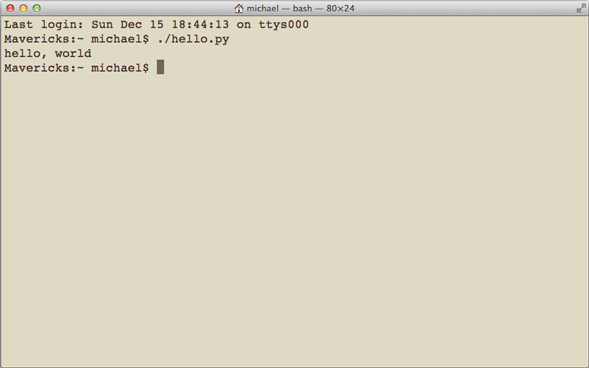
\includegraphics[width=0.6\linewidth]{fig/9236263761773440.png}
\end{figure}


\hypertarget{ux5c0fux7ed3}{%
\subsubsection{小结}\label{ux5c0fux7ed3}}

用文本编辑器写 Python 程序,然后保存为后缀为\texttt{.py}的文件,就可以用
Python 直接运行这个程序了。

Python 的交互模式和直接运行\texttt{.py}文件有什么区别呢?

直接输入\texttt{python}进入交互模式,相当于启动了 Python
解释器,但是等待你一行一行地输入源代码,每输入一行就执行一行。

直接运行\texttt{.py}文件相当于启动了 Python
解释器,然后一次性把\texttt{.py}文件的源代码给执行了,你是没有机会以交互的方式输入源代码的。

用 Python
开发程序,完全可以一边在文本编辑器里写代码,一边开一个交互式命令窗口,在写代码的过程中,把部分代码粘到命令行去验证,事半功倍!前提是得有个
27'的超大显示器!

\hypertarget{ux53c2ux8003ux6e90ux7801}{%
\subsubsection{参考源码}\label{ux53c2ux8003ux6e90ux7801}}

\href{https://github.com/michaelliao/learn-python3/blob/master/samples/basic/hello.py}{hello.py}

